\PassOptionsToPackage{dvipsnames}{xcolor}
\documentclass{beamer}
\usepackage{xcolor}
\usepackage{pgfpages}

\usepackage[style=authortitle]{biblatex}

\setbeameroption{show notes on second screen}

\usepackage[utf8]{inputenc}
\usepackage[T1]{fontenc}
\usepackage{lmodern}
\usepackage{fontawesome}

\usepackage{minted}

\usepackage{listings}

\usepackage[american]{babel}

\usepackage{
    amsmath,
    amsfonts,
    amssymb
}

\usepackage[os=win]{menukeys}

\usetheme{UOS}

\graphicspath{{img/}}

% use this with \begin{pythoncode} ... \end{pythoncode}
\newminted{python}{linenos=false}

\newminted[outputcode]{text}{linenos=false}

% this gets rid of red boxes around syntax errors in minted
\AtBeginEnvironment{minted}{%
  \renewcommand{\fcolorbox}[4][]{#4}}

% removes the prefix "Figure 1:" in figure captions
\setbeamertemplate{caption}{\raggedright\insertcaption\par}


\begin{document}

\title[Strings]{Week 5: Strings}
\subtitle{Basic Programming in Python}

\author[kgross, mpoemsl, sselbach]{Katharina Groß, Martin Pömsl, Sören Selbach}

% change to date of actual lecture
\date{\today}

\begin{frame}[plain]
    \titlepage
\end{frame}

\begin{frame}
    \tableofcontents
\end{frame}


\section{Recap: Lists}

\begin{frame}[plain]
    \sectionpage
\end{frame}

\begin{frame}[fragile]{List Slicing}

    \textbf{Task: Print only the last three elements of a list}

    \begin{pythoncode}

my_list = [1, 2, 3, 4, 5]
print(my_list[-3:])

# Output: [3, 4, 5]

    \end{pythoncode}

    \note{
        This is called \texttt{slicing}.
    }

\end{frame}

\begin{frame}[fragile]{List Comprehension}

    \textbf{Task: Solve the Wheat and Chessboard Problem}

    \begin{pythoncode}

result = sum([2 ** n for n in range(64)])

print([2 ** n for n in range(64)])
# Output: [1, 2, 4, 8, 16, ...]

print([n for n in range(64)])
# Output: [0, 1, 2, 3, 4, ...]

print([2 for n in range(64)]
# Output: [2, 2, 2, 2, 2, ...]
    \end{pythoncode}

    \note{
        Everything that can be done with List Comprehension can also be done with a \texttt{for}-loop, so don't worry if you don't understand it right away.
    }

\end{frame}

\begin{frame}[fragile]{List Comprehension}

    \textbf{Task: Filter a list for odd or even numbers}

    \begin{pythoncode}

original_list = [1, 7, 8, 2, 3]

odd_only = [n for n in original_list if n % 2 != 0]

print(odd_only)
# Output: [1, 7, 3]

even_only = [n for n in original_list if n % 2 == 0]

print(even_only)
# Output: [8, 2]

    \end{pythoncode}

    \note{
        It is also possible to include an \texttt{else} instruction.
    }


\end{frame}

\begin{frame}[fragile]{Strings as Lists of Characters}

    \begin{pythoncode}

my_string = "banana"

print(len(my_string))
# Output: 6

print(my_string[-3:])
# Output: ana

print(sorted(my_string))
# Output: ['a', 'a', 'a', 'b', 'n', 'n']

print([c for c in my_string if c != 'a'])
# Output: ['b', 'n', 'n']

    \end{pythoncode}

    \note{
        Note that the return value of \texttt{sorted(my\_string)} is a list, not a string.
    }
    

\end{frame}

\begin{frame}[fragile]{Strings as Lists of Characters}

    \begin{pythoncode}

my_string = "banana"

for character in my_string:
    print(character)

# Output:
# b
# a
# n
# a
# n
# a

    \end{pythoncode}
    
    \note{
        The variable "character" will be assigned the value of the current character 
        in each iteration of the \texttt{for}-loop.
    }

\end{frame}

\begin{frame}[fragile]{Unicode Table}

	\includegraphics[width=0.9\textwidth]{05_Strings/unicode_table.png}

    \note{
        You can find the full unicode table here:

        \vspace{1em}

        \url{http://www.tamasoft.co.jp/en/general-info/unicode-decimal.html}
    }

\end{frame}

\begin{frame}[fragile]{Calculating with Characters}

    \textbf{The unicode table assigns a unique decimal number to each character.}

    \vspace{1em}    

    We can use \texttt{ord} to get the corresponding \texttt{int} of a character and \texttt{chr} to get the corresponding character of an \texttt{int} in Python.

    \vspace{1em}

    \centering \includegraphics[width=0.5\textwidth]{05_Strings/unicode_table.png}

    \note{
        You can find the full unicode table here:

        \vspace{1em}

        \url{http://www.tamasoft.co.jp/en/general-info/unicode-decimal.html}
    }


\end{frame}


\begin{frame}[fragile]{Calculating with Characters}

    \begin{pythoncode}

print(ord('a')) 
# Output: 97

print(chr(97))
# Output: a

print('a' + 1)
# TypeError: can only concatenate str (not "int") to str

print(chr(ord('a') + 1))
#     chr(97       + 1)
#     chr(98)
# Output: b

    \end{pythoncode}

    \note{

        Hint: This is particularily relevant for the Caesar Cipher task.

        \vspace{1em}
    
        When working with letters, one must make sure not to "drop off" one end of the Latin letters.
    
        \vspace{1em}

        For example, if you try to increase the letter "z" by 1 with this method, you will 
        instead end up at "\{" since this is the next cell in the unicode table.

        \vspace{1em}

        So you have to find a way to make sure that when the result of \texttt{ord(my\_letter) + 1} is greater than 122, 
        it will start counting at 97 again. 

    }

\end{frame}


\section{Creating Strings}

\begin{frame}[plain]
    \sectionpage
\end{frame}

\begin{frame}[fragile]{Creating Strings}

    \begin{enumerate}
        \item Explicitly, e.g. \texttt{my\_string\_1 = "banana"}
        \item Casting, e.g. \texttt{my\_string\_2 = str(97)}
        \item Creating a character, e.g. \texttt{my\_string\_3 = chr(97)}
        \item Special String functions, \newline e.g. \texttt{my\_string\_4 = 'a'.join(['b', 'n', 'n'])}
    \end{enumerate}

    \begin{pythoncode}
# Output of print(my_string_1): banana
# Output of print(my_string_2): 97
# Output of print(my_string_3): a
# Output of print(my_string_4): banan
    \end{pythoncode}

    \note{
        The most common way is to explicitly define them. \texttt{join} will also be explained later on.
    }


\end{frame}


\section{Formatting Strings}

\begin{frame}[plain]
    \sectionpage
\end{frame}

\begin{frame}[fragile]{\texttt{format}}

    \texttt{format} can be used to insert values into a string without the usage of string concatenation with +.

    \begin{pythoncode}
n = 1
my_string = "Hello! This is example number {}.".format(n)

print(my_string)
# Output: Hello! This is example number 1.

print("After example {} comes example {}.".format(1, 2))
# Output: After example 1 comes example 2.

    \end{pythoncode}

    \note{
        For more information about \texttt{format} syntax, see:
    
        \vspace{1em}

        \url{https://docs.python.org/3.7/library/string.html\# format-string-syntax}
    }



\end{frame}

\begin{frame}[fragile]{\texttt{format}}

    It is also possible to index the arguments of \texttt{format} and use them multiple times.

    \begin{pythoncode}

print("I am {1}, so I {0}.".format("eat", "hungry"))
# Output: I am hungry, so I eat.

print("{0} + {0} = {1}".format(1, 2))
# Output: 1 + 1 = 2

print("{season_1} goes, {season_2} comes".format(
    season_1="winter", 
    season_2="spring"
))
# Output: winter goes, spring comes

    \end{pythoncode}

    \note{

        The indexing follows the same system as with lists: 

        \vspace{1em}
    
        The first element is at index 0, the second at index 1, ...
    }


\end{frame}


\begin{frame}[fragile]{\texttt{format}}

    There is even a whole mini language surrounding the use of \texttt{format}. For our purposes, however, it is enough to know how to use fixed-point notation.

    \begin{pythoncode}
result = 2 ** 0.5 # square root of 2

print("The result is {0}.".format(result)
# Output: The result is 1.4142135623730951.

print("The result is {0:.4f}.".format(result)
# Output: The result is 1.4142.

print("The result is {0:.2f}.".format(result)
# Output: The result is 1.41.
    \end{pythoncode}

    \note{
        For more information about \texttt{format} syntax, see:
    
        \vspace{1em}

        \url{https://docs.python.org/3.7/library/string.html\# format-string-syntax}
    }

\end{frame}

\section{Handling Whitespace}

\begin{frame}[plain]
    \sectionpage
\end{frame}


\begin{frame}[fragile]{Whitespace Characters}
    
    \begin{enumerate}

    \item \texttt{\textbackslash n} inserts a linebreak
    \item \texttt{\textbackslash t} inserts a tab
    \item The length of a tab is system dependent (2, 4 or 8 spaces)
    \item A regular space " " is of course also a whitespace character
    \item \texttt{isspace()} can be used to check if a character is a whitespace

    \end{enumerate}

    \begin{pythoncode}

my_string = "a\nb\tc"

print(my_string)
# Output:
# a
# b    c
    
    \end{pythoncode}

    \note{
        There are a lot more whitespace characters, but those are the most relevant ones for our purposes.
    }

\end{frame}

\begin{frame}[fragile]{Whitespace Characters}
    
    \begin{pythoncode}

my_string = "a \nb\tc"

for character in my_string:
    print(character.isspace())

# Output:
# False
# True
# True
# False
# True
# False
    
    \end{pythoncode}

    \note{
        \texttt{isspace} checks for all whitespace characters (not only the ones we know).
    }

\end{frame}



\begin{frame}[fragile]{Removing Whitespace}

    \textbf{There are three main functions to remove whitespace:}

    \begin{enumerate}

    \item \texttt{strip} removes all whitespace characters to the left and right of a string
    \item \texttt{split} divides a string on all whitespace characters and returns a list of the parts
    \item \texttt{splitlines} divides a string on all linebreaks and returns a list of lines

    \end{enumerate}

    \note{

        \texttt{split} and \texttt{join} in combination can be really useful.

    }

\end{frame}


\begin{frame}[fragile]{Removing Whitespace}

    \begin{pythoncode}

my_string = "\tEnjoy the \n sun !  ! !\n"

print(my_string)
# Output:
#	 Enjoy the 
# sun !  ! !
# 

print(my_string.strip())
# Output:
# Enjoy the 
#  sun !  ! !

    \end{pythoncode}

\end{frame}

\begin{frame}[fragile]{Removing Whitespace}

    \begin{pythoncode}
my_string = "\tEnjoy the \n sun !  ! !\n"

print(my_string.split())
# Output: ['Enjoy', 'the', 'sun', '!', '!', '!']

print(my_string.splitlines())
# Output: ['\tEnjoy the ', ' sun !  ! !']

# We can merge the resulting lists together with join

print(" ".join(my_string.split()))
# Output: Enjoy the sun ! ! !

    \end{pythoncode}

\end{frame}



\begin{frame}[fragile]{Excursion: Whitespace in Python}
	
    \centering 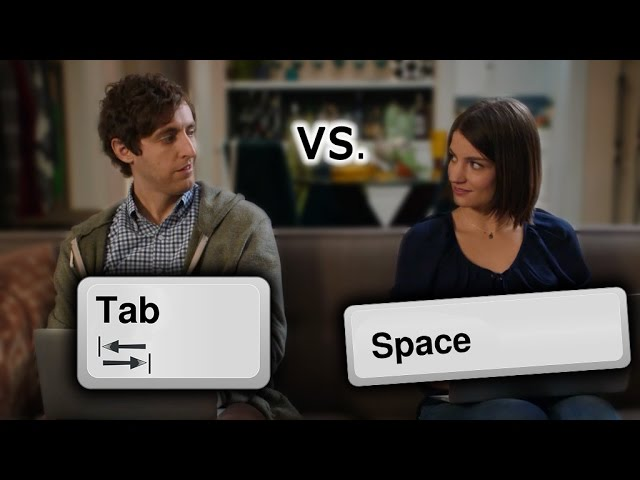
\includegraphics[width=0.75\textwidth]{05_Strings/tabs_vs_spaces.jpg}

    \note{
        The picture is taken from an episode of the series Silicon Valley, which depicts the struggle of programmers in California in a funny way.

        \vspace{1em}

        The referred scene about the whole "Tabs vs. Spaces" argument can also be found on YouTube.

    }

\end{frame}

\begin{frame}[fragile]{Excursion: Whitespace in Python}
	
    In Python, we use whitespace to \textbf{indent blocks of code}. 
    These can either be produced using tabs or spaces.
    If you mix them in your Python code, you will get an \texttt{IndentationError}.
    
    
    \begin{pythoncode}

if my_condition:
    print(my_old_variable)
    my_new_variable = my_old_variable + 1
    print(my_new_variable)

print(my_condition)

    \end{pythoncode}

    \textbf{In this course, we ask you to use four spaces just so we can all edit and execute each other's code.}

    \note{
        
        Having the same convention about tabs and spaces is particularily important when collaborating on a project with other programmers.

    }

\end{frame}


\section{Evaluating Strings}

\begin{frame}[plain]
    \sectionpage
\end{frame}

\begin{frame}[fragile]{Checking Strings}

    There are many functions that check whether a string fulfills a certain condition. They return a boolean value (\texttt{True} or \texttt{False}).

    \vspace{1em}

    They all follow this basic syntax:

    \begin{pythoncode}
        
my_string_1 = "hello people"
my_string_2 = "Hello people"
my_string_3 = "HELLO PEOPLE"

boolean_value = my_string_1.islower()
        
print(boolean_value)
# Output: True

    \end{pythoncode}
    

    \note{
        What is being checked is whether \textbf{all} characters in the string fulfill the condition.

        \begin{enumerate}

        \item \texttt{isalpha} checks if a string is all alphabetic
        \item \texttt{isnumeric} checks if a string is all numeric
        \item \texttt{isalnum} checks if a string is all alphabetic or numeric
        \item \texttt{isupper} checks if a string is all lowercase
        \item \texttt{islower} checks if a string is all uppercase  
        \item \texttt{isspace} checks if a string is all whitspace
        \item \texttt{startswith} checks if a string starts with another string
        \item \texttt{endswith} checks if a string ends with another string

        \end{enumerate}
    }

\end{frame}


\begin{frame}[fragile]{Checking Strings}

    \begin{pythoncode}
        
my_string_1 = "hello people"
my_string_2 = "Hello people"
my_string_3 = "HELLO PEOPLE"

print(my_string_1.islower())
# Output: True

print(my_string_3.islower())
# Output: False

print(my_string_2.islower())
# Output: ???

    \end{pythoncode}
    

    \note{

        What is being checked is whether \textbf{all} characters in the string fulfill the condition.

        \begin{enumerate}

        \item \texttt{isalpha} checks if a string is all alphabetic
        \item \texttt{isnumeric} checks if a string is all numeric
        \item \texttt{isalnum} checks if a string is all alphanumeric
        \item \texttt{isupper} checks if a string is all lowercase
        \item \texttt{islower} checks if a string is all uppercase  
        \item \texttt{isspace} checks if a string is all whitspace
        \item \texttt{startswith} checks if a string starts with another string
        \item \texttt{endswith} checks if a string ends with another string

        \end{enumerate}
    }

\end{frame}


\begin{frame}[fragile]{Evaluating Strings}

    \begin{enumerate}

        \item \texttt{len} can be used to obtain the total number of characters in a string
        \item \texttt{in} can be used to check if a string is contained in another string
        \item \texttt{count} can be used to obtain the number of occurences of a string in another string
        \item \texttt{find} can be used to obtain the index of the first occurence of a string in another string

    \end{enumerate}

    \note{
        
        All of these functions return an \texttt{int}.

        \vspace{1em}

        You can find the indices of multiple occurrences by applying \texttt{find} multiple times, 
        specifying the start index and increasing in after each found index.

        \vspace{1em}

        More information on \texttt{find} can be found here:

        \vspace{1em}

        \url{https://docs.python.org/3/library/stdtypes.html\# str.find}

    }


\end{frame}

\begin{frame}[fragile]{Evaluating Strings}

    \begin{pythoncode}

my_string = "the quick brown fox jumps over the lazy dog"

print(len(my_string))
# Output: 43

print("fox" in my_string)
# Output: True

print("banana" in my_string)
# Output: False

    \end{pythoncode}

    \note{
        \texttt{in} can also be used on lists.
    }

\end{frame}

\begin{frame}[fragile]{Evaluating Strings}

    \begin{pythoncode}

my_string = "the quick brown fox jumps over the lazy dog"

print(my_string.count("fox"))
# Output: 1

print(my_string.count("the"))
# Output: 2

print(my_string.find("the"))
# Output: 0

    \end{pythoncode}

     \note{
        \texttt{count} can also be used on lists.
    }

\end{frame}

\section{Modifying Strings}

\begin{frame}[plain]
    \sectionpage
\end{frame}

\begin{frame}[fragile]{Immutability}

    \textbf{Strings are immutable}, so despite their similarities with lists they cannot be changed.

    \begin{pythoncode}

my_string = "banana"

print(my_string[2])
# Output: n

my_string[2] = 'i'
# TypeError: 'str' object does not support item assignment
    
    \end{pythoncode}

    \note{
         Like \texttt{tuples}, strings can be indexed, but not changed. So all functions that appear to change a string in fact just return a changed copy.
    }

\end{frame}

\begin{frame}[fragile]{Changing Case}

    These functions change the capitalization of the words in a string:

    \begin{enumerate}

        \item \texttt{upper} can be used to make all characters uppercase
        \item \texttt{lower} can be used to make all character lowercase
        \item \texttt{title} can be used to make all words title case

    \end{enumerate}

    \begin{pythoncode}

my_string = "hello, How are YOU?"

my_string_lower = my_string.lower()
my_string_upper = my_string.upper()

print(my_string, my_string_lower, "\n", my_string_upper)
# Output: hello, How are YOU? hello, how are you? 
#          HELLO, HOW ARE YOU?

    \end{pythoncode}

    \note{

        For properties like cases there always exists a pair of functions such that:

        \vspace{1em}

        \texttt{my\_string.property()} transforms the string to have this property.
    
        \vspace{1em}

        \texttt{my\_string.isproperty()} returns a boolean whether as the string has this property.
    
    }

\end{frame}

\begin{frame}[fragile]{\texttt{strip}}

    \texttt{strip} can also take an argument and remove an arbitrary string from both sides of a string:

    \begin{pythoncode}

my_string = "banana HELLO banana"

print(my_string.strip("banana"))
# Output: HELLO 
    
    \end{pythoncode}

    There exist functions \texttt{rstrip} and \texttt{lstrip} as well to apply this to only one side of the string.

    \note{
        \texttt{rstrip} strips from the right side, \texttt{lstrip} from the left side.
    }
    

\end{frame}

\begin{frame}[fragile]{\texttt{split} and \texttt{join}}

    \texttt{split} can split on a custom string as well:

    \begin{pythoncode}

my_string = "banana HELLO banana"

print(my_string.split(" HELLO "))
# Output: ['banana', 'banana']
    
    \end{pythoncode}

    Using this in combination with \texttt{join}, it is possible to replace all occurences of a string with another string. 

    \vspace{1em}

    However, for this there also exists a specialized function \texttt{replace}.
    

\end{frame}

\begin{frame}[fragile]{\texttt{split} and \texttt{join}}

    \textbf{Task: Replace all occurences of "Tom" with another name.}

    \begin{pythoncode}

my_string = """One day there was a baker named Tom. 
Tom liked to bake a lot of breads. """

my_string_splitted = my_string.split("Tom")
print(my_string_splitted)
# Output: ['One day there was a baker named ', 
# '. \n', ' liked to bake a lot of breads. ']

my_string_joined = "Mary".join(my_string_splitted)
print(my_string_joined)
# Output: One day there was a baker named Mary. 
# Mary liked to bake a lot of breads.

    \end{pythoncode}

    \note{
        The triple quotation mark """ can be used to start and end multiline strings. Multiline strings are strings that span more than one line of text.
    }

\end{frame}

\begin{frame}[fragile]{\texttt{replace}}

    \textbf{Task: Replace all occurences of "Tom" with another name."}

    \begin{pythoncode}

my_string = """One day there was a baker named Tom. 
Tom liked to bake a lot of breads. """

my_string_replaced = my_string.replace("Tom", "Mary")

print(my_string_replaced)
# Output: One day there was a baker named Mary. 
# Mary liked to bake a lot of breads.

    \end{pythoncode}

\end{frame}

\section{Outlook: RegEx}

\begin{frame}[plain]
    \sectionpage
\end{frame}

\begin{frame}[fragile]{Outlook: RegEx}

    \textbf{Regular Expressions} are a powerful tool to replace not just predefined strings, but any string that matches a pattern. 

    \begin{pythoncode}

import re

re_example = re.compile("[0-9]")

my_string = "Guido van Rossum (born 31 January 1956) ..."

print(re_example.sub("X", my_string))
# Output: Guido van Rossum (born XX January XXXX) ...

    \end{pythoncode}

    \note{
        Learn more about RegEx here: 

        \vspace{1em}

        \url{https://docs.python.org/3/howto/regex.html}
    }

\end{frame}

\begin{frame}[fragile]{Outlook: RegEx}

    \begin{pythoncode}

re_example_1 = re.compile("[a-z]")
re_example_2 = re.compile("[a-b]")
re_example_3 = re.compile("van|born")

print(re_example_1.sub("X", my_string))
# Output: GXXXX XXX RXXXXX (XXXX 31 JXXXXXX 1956) ...

print(re_example_2.sub("X", my_string))
# Output: Guido vXn Rossum (Xorn 31 JXnuXry 1956) ...

print(re_example_3.sub("X", my_string))
# Output: Guido X Rossum (X 31 January 1956) ...

    \end{pythoncode}

    \note{
        Learn more about RegEx here: 

        \vspace{1em}

        \url{https://docs.python.org/3/howto/regex.html}

        \vspace{1em}

        Especially if you are interested in working with text data, RegEx is an invaluable and powerful tool.

        \vspace{1em}

        The whole syntax is much more sophisticated than what is covered on these slides.
    }

\end{frame}

\end{document}
